\section {Stadiul actual al tehnologiilor utilizate pentru dezvoltarea solu'tiei}

Dezvoltarea unui sistem \acrshort{iot} de automatizare presupune atât o parte hardware cât 'si una software. Pentru controlarea hardware-ului de la distan'tă este nevoie de un canal de comunica'tii prin care să se i trimi'tă comenzi. În general, în cazul sistemelor embedded de acest tip folosesc un microcontroller sau un microprocesor care implementează stiva \acrshort{ip}.

O altă abordare populară în proiectarea acestor sisteme este dezvoltarea unui controller conectat la internet care are rolul de a colecta informa'tii de la alte dispozitive din incintă compatibile cu protocolul sau. Mai departe, informa'tiile colectate sunt transmise unui server spre a fi preprocesate, agregate, oferind utilizatorului date relevante momentului respectiv.

În func'tie de complexitatea solu'tiei, partea responsabilă pentru procesarea evenimentelor poate varia de la un simplu server conectat la o bază de date până la un cluster de big-data compus din sute de noduri capabile să ruleze algoritmi de agregare distribui'ti.


\subsection {Apple, Amazon, Google}

Potrivit articolului \cite{AppleRebuildsSiriMesos}, Apple folose'ste Apache Mesos, un manager open-source pentru clustere de computa'tie capabil să scaleze până la zeci de mii de noduri pentru a rula serviciile necesare asistentului inteligent Siri într-o manieră care oferă redundan'tă la eroare. Următorul nivel de integrare vine de la compania Amazon, care rulează algoritmii asistenutlui sau inteligent Alexa pe platforma sa de servicii web, \acrfull{aws}. Într-o manieră similară putem specula că o companie precum Google folose'ste tehnologia sa de orchesterare pentru clustere de computa'tie, Kubernetes, pentru a rula serviciile necesare Google Assistant.

Toate aceste solu'tii includ integrări cu sisteme \acrshort{iot} precum lumini inteligente, aspiratoare autonome sau încuietori inteligente au o complexitare ridicată, justificând necesitatea unui cluster computa'tional distribuit. 

\subsection {Espressif}

Espressif Systems oferă o abordare alternativă problemei, prin protocolul de comunica'tii Esspressif care compactează 5 layere din stiva \acrfull{osi} într-unul singur, reducând latenta cauzată de pierderea pachetelor în re'tele congestionate. Fiind mai simplu, irose'ste mai pu'tini cicli ai microprocesorului 'si consumă mai pu'tină memorie. Pentru a permite interac'tiunea senzorilor 'si actorilor Esspressif cu dispozitive mobile care nu implementează acest protocol este nevoie de un gateway care să realizeze traducerea pachetelor intre cele doua re'tele, însă acest lucru este op'tional.

\begin{figure}[h!]
  \centering
  \fbox {
    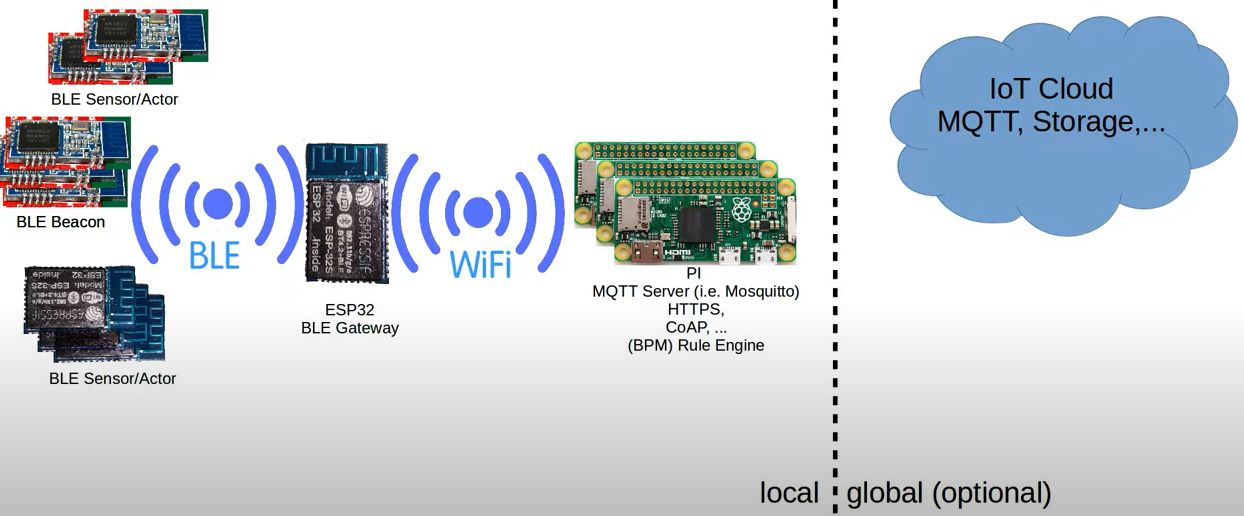
\includegraphics[width=\singlephoto]{03/01_espressif_gateway.png}  
  }
  \caption{Sistem interconectare actori Espressif la internet \cite{StackOverflow2021Espressif}}
\end{figure}

Din perspectiva utilizatorului, dispozitivele noi necesită un pas de împerechere în re'tea, după fiind complet autonome. Chiar dacă frameworkul oferă func'tii ajutătoare pentru criptarea informa'tiilor transmise, aplica'tiile pot alege să implementeze metoda standard Curve25519, să î'si implementeze propriul mecanism sau chiar să îl dezactiveze complet.

Compania din spate oferă printre altele 'si o familie de microcontrollere numită ESP, gândită pentru a accelera procesul de dezvoltare a noi senzori 'si actori în re'tea, oferind o gamă largă în materie de conectivitate.

\subsection {Solu'tia hobbyista}

Proiectandu-ne propriul sistem, beneficiem de libertate în modelarea problemei 'si alegerea protocoalelor de comunicare. A'sadar, se poate concepe un sistem \acrshort{iot} care să ofere un set de func'tionalită'ti mai restrâns, folosind hardware disponibil consumatorilor de rând 'si tehnologii software open-source.

Adi'tional, pentru o integrare minimală cu unul din asisten'tii personali men'tiona'ti mai sus, de obicei este pus la dispozi'tia dezvoltatorilor un API bazat pe webhook-uri. Acesta sarcină presupune implementarea unor servicii \acrshort{rest} pe baza unor specificiatii prestabilite. 

\section {Prezentarea tehnologiilor 'si platformelor de dezvoltare alese}

\subsection {Hardware}

Deoarece proiectul necesita atât interac'tiunea cu sisteme electrice cât 'si cu sisteme digitale precum stiva \acrshort{ip}, am ales placa de dezvoltare "Raspberry Pi 3 Model B Rev 1.2". Aceasta oferă un procesor quad core cu arhitectura armv7 de 1.2 Ghz, 1 GB RAM 'si 26 de pini \acrfull{gpio} pentru interac'tiunea cu terminalul \acrshort{pots}.

Considerând complexitatea relativ scăzută a circuitului electric, pentru proiectarea \acrshort{pcb} am ales Fritzing, un soft open-source de \acrfull{cad}. Spre deosebire de un program mai profesionist precum Eagle, Fritzing este u'sor de folosit 'si dispune de o librărie care con'tine majoritatea componentelor anologice 'si digitale. În cazul în care nu exista model pentru o componenta, utilizatorul are posibilitatea de a crea un model din poze 'si măsurători. 

\subsection {Backend}

Într-un studiu anual realizat de Stack Overflow, peste 80,000 de dezvoltatori software au ales JavaScript ca cel mai folosit limbaj de programare pentru al nouălea an consecutiv. NodeJS a urcat pe locul 5 în popularitate, în timp ce Typescript este pe locul 6. Datorită cerin'tei de portabilitate am ales NodeJS ca limbaj pentru implementarea serverului aplica'tiei. \cite{StackOverflow2021Survey}

Printre alternative viabile pentru acest tip de proiect se numără Java, C\# sau Python, limbaje aflate în primele 10 în topul celor de la Stack Overflow.

Ca framework de dezvoltare a serverului am ales NestJS, oferind o arhitectura \acrfull{mvc} 'si multe func'tionalită'ti convenabile precum:

\begin{itemize}
  \item Framework de injectare a dependin'telor: graful (aciclic) de dependin'te al aplica'tiei este calculat la pornire, fiecărui modul îi sunt satisfăcute dependin'tele, instantiindu-se obiectele necesare o singura data. Daca sunt detecta'ti cicli în graful de dependin'te sau nu exista informa'tii despre cum se poate instantia o clasa, atunci se va arunca o eroare de runtime 'si aplica'tia va ie'si cu un status code de eroare. 
  \item Separarea logicii de control a aplica'tiei de interfa'tă 'si de date. Utilizatorul interac'tionează cu interfa'tă, care notifică controllerul de ac'tiunile utilizatorului, controllerul execută logica aplica'tiei 'si actualizează modelul corespunzător, schimbări ce se vor reflecta în interfa'tă.
  \item Îmbină elemente de \acrfull{oop}, \acrfull{fp} 'si \acrfull{frp}. De exemplu: modulele 'si serviciile sunt clase, iar decoratorii claselor sunt func'tii care modifică comportamentul func'tiilor adnotate prin compunere.

\end{itemize}

\subsection {Baza de date}

Din punct de vedere al scalabilitatii, pradigma rela'tională scaleaza vertical (pu'tine servere puternice), pe când cea nerelationala este orizontală (multe servere mici). Prin urmare se va utiliza MongoDB, o solu'tie de tip NoSQL rulată în modul "cluster" pentru a oferi redundan'tă datelor prin replicarea lor de 3 ori pe noduri diferite fizic.

Deoarece MongoDB are nevoie de suport pentru 64 bi'ti, nu poate fi instalată pe acela'si Raspberry Pi unde va rula 'si serverul. Pentru simplitudine, s-a ales un serviciu online de hosting gratis, numit Mongo Atlas. A'sadar, serverul NodeJS trebuie să 'tină cont de eventuala laten'tă mai ridicată în comunicarea cu baza de date 'si retransmiterea comenzilor în cazul în care niciunul din nodurile clusterului nu este disponibil.

\noindent
\textit{Object Document Mapping}

Pentru transformarea 'si validarea obiectelor de JavaScript în documente ce vor fi stocate în baza de date, am ales Mongoose.


\subsection {Firebase Cloud Messaging}

Pentru transmiterea notificărilor 'si evenimentelor în timp real către dispozitive mobile s-au luat în calcul mai multe solu'tii de tip Pub/Sub, însă solu'tia finala aleasa a fost Firebase, datorită stabilită'tii ridicate prin integrarea strânsă cu sistemul de operare. În spate, se folosesc Google Play Services pentru a se livra informa'tiile utilizatorului într-o manieră eficientă, sistemul putând să  întârzie u'sor evenimentele pentru trezi cât mai pu'tin procesorul dispozitivului notificat \cite{FirebaseGoogle2022}.

Alte solu'tii investigate au fost OneSignal 'si MQTT, cel din urma fiind folosit de Facebook în aplica'tia lor de mesagerie \cite{LucyZhang2021}. Acest protocol a fost proiectat pentru a trimite date de telemetrie de la sonde din spa'tiu, men'tinând consumul de baterie 'si lă'timea de banda la minim. Chiar dacă acest sistem prezintă anumite avantaje, complexitatea ridicată de implementare a fost factorul care a influen'tat decizia finală de a de a folosi Firebase. 

\subsection {Client}

Android este o platformă mobilă care s-a maturizat pe parcusul a 12 versiuni majore 'si principalul competitor de pia'tă al iOS. Având experien'tă anterioară ca programator Android 'si în special cu limbajul de programare Java, a fost o alegere convenabilă pentru un prototip rapid.
Este de men'tionat că aceasta alegere de platforma este pur subiectivă, un client similar putând fi dezvoltat pentru iOS sau cu o tehnologie care suportă cross-compilation cum ar fi React Native sau Ionic.
